\documentclass[10pt, spanish]{article}
\usepackage[spanish, activeacute]{babel}
\usepackage[latin1]{inputenc}
\usepackage{graphicx}

\begin{document}
\title{Universidad Sim�n Bol�var \\ Inteligencia II \\ Tarea 1}
\author{
  Daniel Barreto - \#04-36723 \texttt{<daniel.barreto.n@gmail.com>} \\
  Kristoffer Pantic - \#05-38675 \texttt{<kristoffer.pantic@gmail.com>}
}
\maketitle

\section{Resumen}
\label{sec:resumen}
blabla

\section{Detalles de Implementaci�n}
\label{sec:di}
Para la realizaci�n de los puntos de la tarea se crearon cuatro tipos
abstractos de datos y algunas funciones auxiliares:

\subsection{Tipos abstractos de datos}

\textbf{Perceptron}\\
Esta clase representa una red neural sin capaz escondidas y �nicamente
con una neurona de salida, que mantiene un vector de pesos para cada
input que recibe. En esta clase se encuentran los m�todos necesarios
para evaluar el resultado de un vector de inputs y para entrenarse con
un conjunto de prueba.

La evaluaci�n devuelve un n�mero real que est� dado como el producto
punto del vector de inputs y el vector de pesos\\

\textbf{BooleanPerceptron}\\
Esta clase hereda de la clase \emph{Perceptron}, pero sobreescribe la
forma en la que se realiza la evaluaci�n de los inputs para
representar la evaluaci�n de una funci�n \emph{threshold} y devolver
�nicamente 0 cuando la evaluaci�n real d� un n�mero no positivo,
o 1 en el caso contrario.\\

\textbf{SigmoidNeuron}\\
Hereda igualmente de la clase \emph{Perceptron} para obtener su
atributo b�sico de la lista de pesos asociados a una lista de
inputs. La diferencia entre \emph{SigmoidNeuron} y \emph{Perceptron}
se encuentra en la evaluaci�n de un input dado, para el cual
\emph{SigmoidNeuron} retorna la funci�n sigmoidal aplicada sobre el
producto punto del vector de pesos y el vector de inputs.\\

\textbf{NeuralNetwork}\\
Utiliza SigmoidNeuron para generar las instancias de todas las
neuronas que conforman la red. Posee 3 atributos: \emph{n�mero de
  inputs}, \emph{lista de neuronas de la capa intermedia}, \emph{lista
  de neuronas de la capa de salida}.  Con dichos atributos se define
el entrenamiento con \emph{backpropagation} como un m�todo de la clase
d�nde se utilizan listas de listas de pesos en vez de una matriz de
pesos para representar las fuerzas de las
conexiones entre cada neurona.\\

\subsection{Funciones Auxiliares}
\textbf{\texttt{training(neural\_network, training\_set,
    learning\_rate=.1,\\ max\_iterations=1000, reduce\_rate=False)}}\\
Es la funci�n principal del programa al momento de entrenar una red
neural, se encarga de realizar un m�ximo de iteraciones
(\texttt{max\_iterations}) sobre un conjunto de entrenamiento
(\texttt{training\_set}) dado, d�nde en cada iteraci�n se le pide a la
red neural (\texttt{neural\_network}) que entrene con
\emph{backpropagation} utilizando una taza de aprendizaje
(\texttt{learning\_rate}) y posiblemente una reducci�n de la misma en
cada iteraci�n (\texttt{reduce\_rate}).\\

\textbf{\texttt{test(neural\_network, test\_set)}}\\
Prueba el rendimiento de una red neural (\texttt{neural\_network})
sobre un conjunto de pruebas (\texttt{test\_set}). Devuelve un par de
listas de puntos; en la primera lista de puntos se encuentran todos
aquellos puntos que forman parte del \emph{�rea A}, y en la segunda
los que forman parte del\emph{�rea B}.\\

A parte de estas funciones, existen otras menos importantes como:\\
\texttt{get\_random\_set(set\_size)},
\texttt{load\_training\_set(file\_name)}, \texttt{plot(error\_log,
  test\_log)} que se utilizan para generar conjuntos random de pruebas,
cargar conjuntos de pruebas desde archivos y graficar la salida del
desempe�o de una red neural, respectivamente.

\section{An�lisis de Resultados}
\label{sec:analisis}

\subsection{Parte 1: Perceptrones}

\subsubsection{Pregunta 1.a}
\begin{figure}[htp]
  \centering
  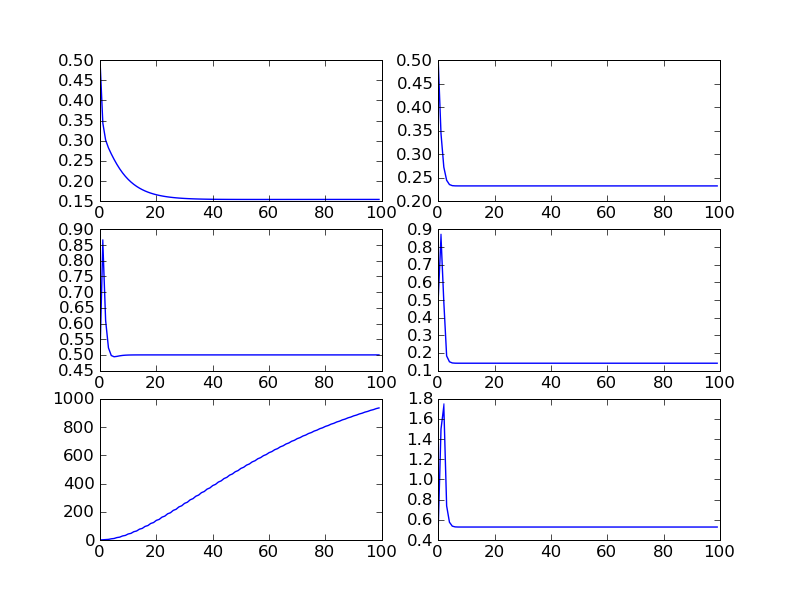
\includegraphics[scale=0.5]{media/p12a-AND.png}
  \caption{Algun caption}\label{fig:nodos}
\end{figure}


\subsubsection{Pregunta 2.a}

\subsubsection{Pregunta 2.b}
Se puede ver que utilizando el aprendizaje por lotes converge m�s
r�pido que el aprendizaje incremental, pero requiere mayor cantidad de
c�mputo por iteraci�n. TIEMPO?

\subsection{Parte 2: Red neural y backpropagation}
Se realizaron entrenamientos con redes de 2 a 10 neuronas en la capa
intermedia sobre los 6 conjuntos especificados en el enunciado. Los
conjuntos utilizados son los siguientes:

\begin{figure}[htp]
  \centering
  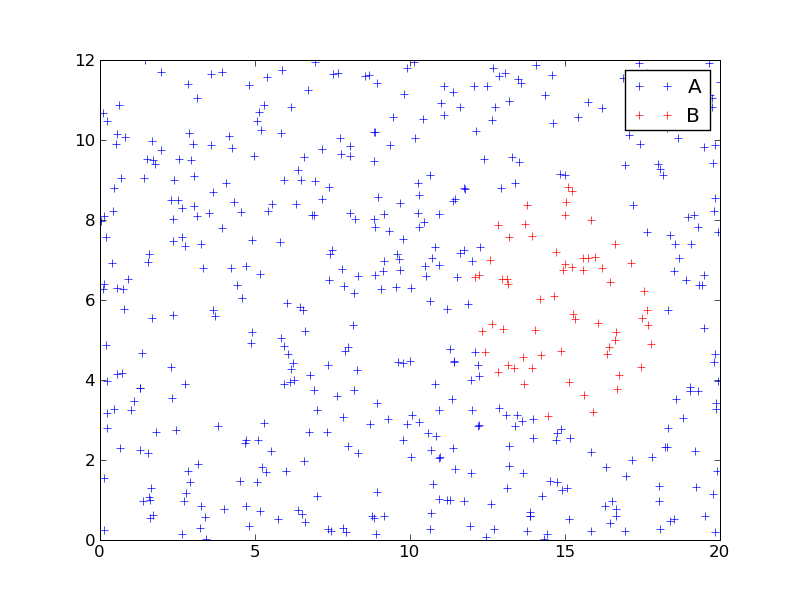
\includegraphics[scale=0.5]{media/500.png}
  \caption{500 puntos uniformemente repartidos}\label{fig:nodos}
\end{figure}

\begin{figure}[htp]
  \centering
  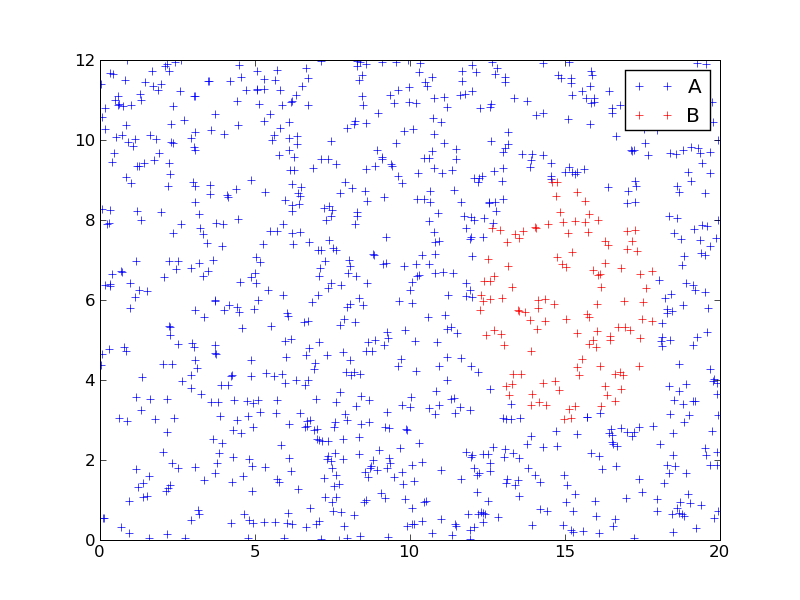
\includegraphics[scale=0.5]{media/1000.png}
  \caption{1000 puntos uniformemente repartidos}\label{fig:nodos}
\end{figure}

\begin{figure}[htp]
  \centering
  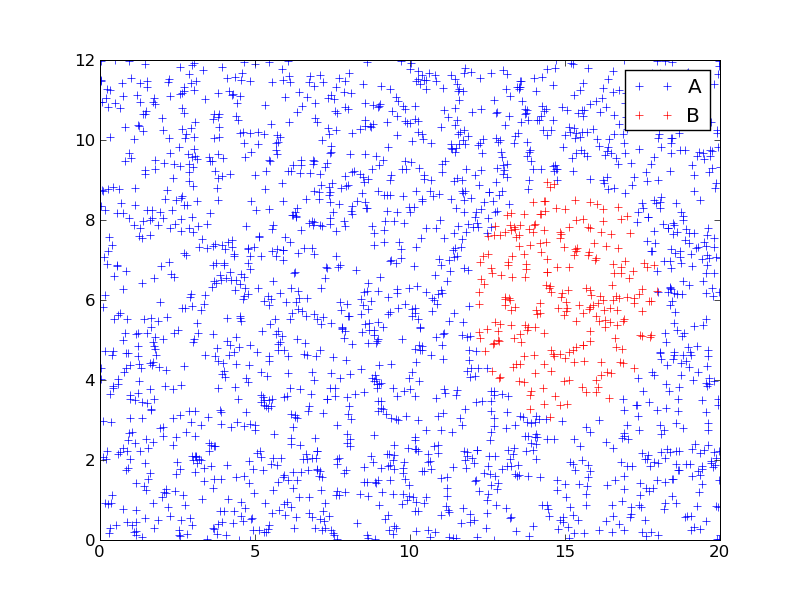
\includegraphics[scale=0.5]{media/2000.png}
  \caption{2000 puntos uniformemente repartidos}\label{fig:nodos}
\end{figure}

\begin{figure}[htp]
  \centering
  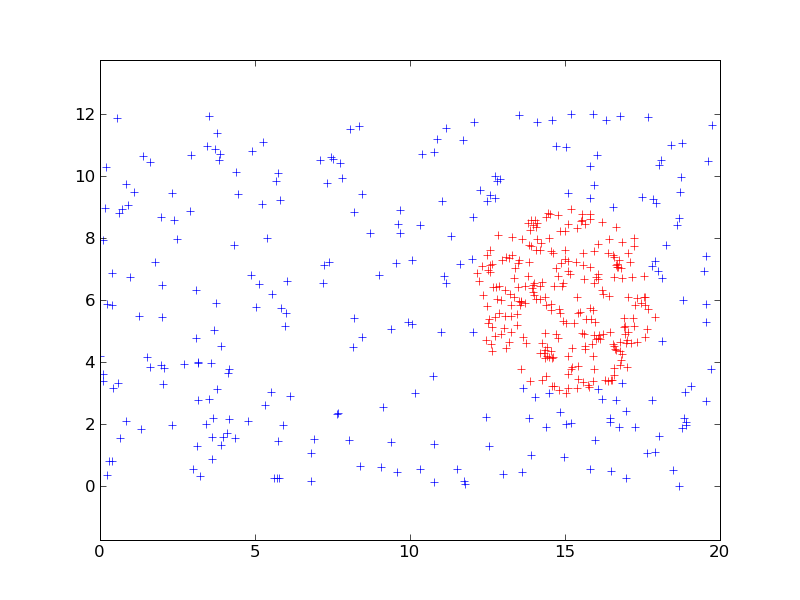
\includegraphics[scale=0.5]{media/500e.png}
  \caption{500 puntos equivalentemente repartidos}\label{fig:nodos}
\end{figure}

\begin{figure}[htp]
  \centering
  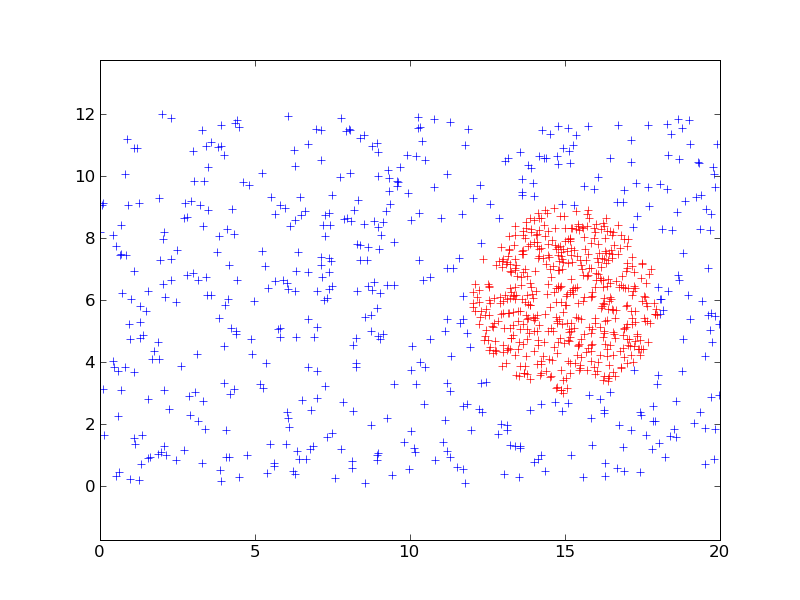
\includegraphics[scale=0.5]{media/1000e.png}
  \caption{1000 puntos equivalentemente repartidos}\label{fig:nodos}
\end{figure}

\begin{figure}[htp]
  \centering
  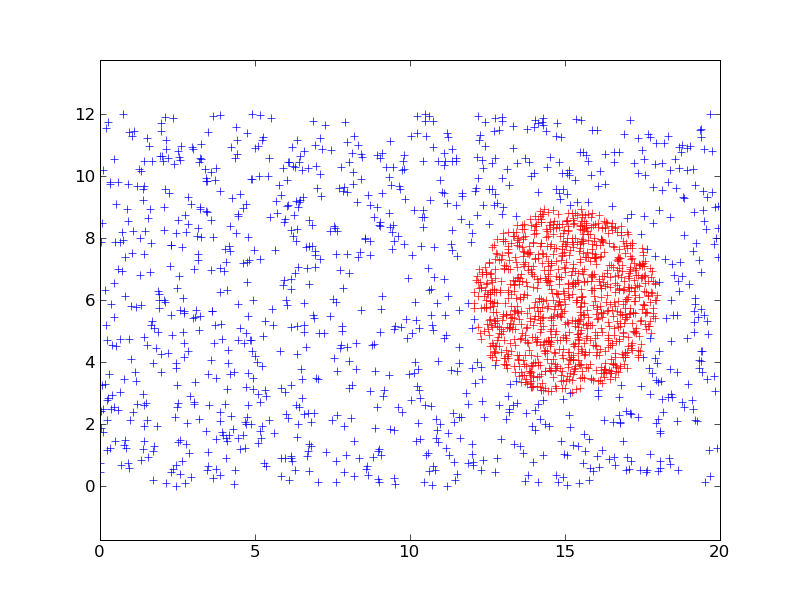
\includegraphics[scale=0.5]{media/2000e.png}
  \caption{2000 puntos equivalentemente repartidos}\label{fig:nodos}
\end{figure}

Los mejores resultados obtenidos en cada conjunto, probando contra
conjuntos de prueba de 10000 puntos generados aleatoriamente sobre
toda la superficie, fueron los siguientes:

\subsection{500 puntos uniformemente repartidos}
Mejor resultado obtenido con \textbf{10 neuronas} intermedias.\\
Porcentaje de error: \textbf{4.48\%}

\subsection{1000 puntos uniformemente repartidos}
Mejor resultado obtenido con \textbf{10 neuronas} intermedias.\\
Porcentaje de error: \textbf{2.7\%}

\subsection{2000 puntos uniformemente repartidos}
Mejor resultado obtenido con \textbf{10 neuronas} intermedias.\\
Porcentaje de error: \textbf{2.7\%}

\subsection{500 puntos equivalentemente repartidos}
Mejor resultado obtenido con \textbf{10 neuronas} intermedias.\\
Porcentaje de error: \textbf{2.7\%}

\subsection{1000 puntos equivalentemente repartidos}
Mejor resultado obtenido con \textbf{10 neuronas} intermedias.\\
Porcentaje de error: \textbf{2.7\%}

\subsection{2000 puntos equivalentemente repartidos}
Mejor resultado obtenido con \textbf{10 neuronas} intermedias.\\
Porcentaje de error: \textbf{2.7\%}

\end{document}